Given the win rates from section~\ref{sec:Methods}
a Shapiro-Wilk's test is applied to each configuration
resulting in the p-values shown in table~\ref{tab:shapiro-wilks}
\begin{table}[H]
	\begin{center}
		\caption{P-values from applying Shapiro-Wilk's test on win rates over $1000$ games}
		\label{tab:shapiro-wilks}
		\begin{tabular}[c]{|c|l|}
			\hline
			Configuration &     p-value             \\ \hline
			C1            &    $1.53\cdot10^{-5}$   \\
			C2            &    $8.01\cdot 10^{-6}$  \\
			C3            &    $4.33\cdot 10^{-5}$  \\
			C4            &    $3.08 \cdot 10^{-5}$ \\ 
			C5            &    $7.47\cdot 10^{-6}$  \\ 
			C6            &    $3.36\cdot10^{-6}$   \\ \hline
		\end{tabular}
	\end{center}
\end{table}
Due to all the p-values presented in table~\ref{tab:shapiro-wilks}
being less than $0.05$, its concluded that all win rate samples
are not normally distributed.
However due to Shapiro-Wilk's test being a non-parametric method designed to test for 
theoretical normality i.e. the perfect bell curve, in large samples these tests are overpowered 
to detect minor deviations from normality, thus false negatives for normality are likely produced.
For this reason a qq-plot is applied to determine the configurations normality. 
The result can be seen in figure~\ref{fig:qqplots}.
\begin{figure}[h]
	\begin{small}
		\begin{center}
			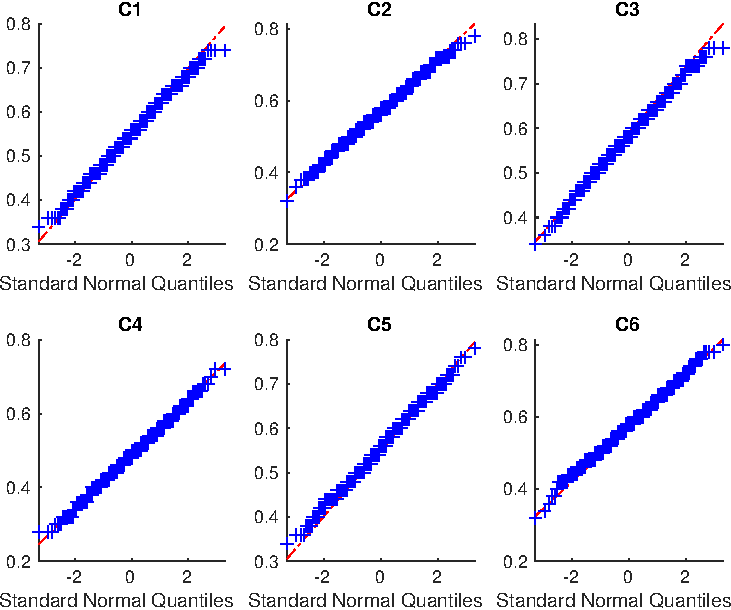
\includegraphics[width=0.7\textwidth]{fig/myfigure.pdf}
		\end{center}
		\caption{qq-plots showing the normality for avg win rates of each configuration}
		\label{fig:qqplots}
	\end{small}
\end{figure}
Based on these results it is concluded that all the average win rates are in fact normally
distributed.
To determine if all the samples have equal variance the Bartlett test was applied which resulted in a 
p-value of approximately $0.897$. Since this value is greater than $0.05$, it is concluded that
 all the avg win rate samples have equal variance.
Finally to test if the configurations perform statistically 
significantly different, a two factor ANOVA is applied 
due to the previous statistical findings. 
The result of this test can be seen in table~\ref{tab:2-factor-anova-table}
\begin{table}[H]
	\begin{center}
		\caption{ANOVA table from an two factor ANOVA test between the crossover rate and selection methods effect on avg win rate}
		\label{tab:2-factor-anova-table}
		\begin{tabular}{|l|l|l|l|l|}
			\hline
			{} &     sum sq &      df &           F &         p-value \\ \hline
			crossover rate                     &   3.98 &     2.00 &  398.68 &   $2.75\cdot 10 ^{-163}$ \\
			selection method                   &   1.15 &     1.00 &  231.70 &   $2.28\cdot 10^{-51}$   \\
			crossover rate:selection method    &   0.95 &     2.00 &   95.80 &   $1.10\cdot 10^{-41}$   \\
			Residual                           &  29.98 &  5994.00 &         &                          \\ \hline
		\end{tabular}
	\end{center}
\end{table}
As it here can be seen the p-values for each tested case rejects the null hypothesis, meaning the 
samples does not come from the same distribution. To determine which configuration performs the best,
each configuration's samples mean is found as shown in table~\ref{tab:mean-and-variance}.
It can here be seen that the best configuration is C3 with a mean avg win rate of $58.3\%$. 
Here a repeated 2 sample t-test is applied between C3 and the other configurations
to determine if there is statistical evidence to support that any of the other configurations 
are from the same distribution, resulting in the p-values presented in table~\ref{tab:2-sample-t-test}.
\begin{table}[!htb]
    \begin{minipage}{.5\linewidth}
		\centering
		\caption{Mean for all configurations C1-C6}
		\label{tab:mean-and-variance}
        \begin{tabular}{|l|l|} \hline
					Conf.         &  Mean  \\ \hline
					C1            &  0.550 \\
					C2            &  0.569 \\
					C3            &  0.583 \\
					C4            &  0.487 \\
					C5            &  0.556 \\
					C6            &  0.577 \\\hline
        \end{tabular}
    \end{minipage}%
	\hspace{0.3cm}
	\begin{minipage}{.5\linewidth}
      \centering
	  \caption{2 sample t-test between C3 \\ and other configurations}
	  \label{tab:2-sample-t-test}
	  	\begin{tabular}{|l|l|l|}\hline
				  Conf. comparison & p-values    \\ \hline
				  C3/C1 & $5.617\cdot 10^{-25 }$ \\
				  C3/C2 & $1.631\cdot 10^{-05 }$ \\
				  C3/C4 & $5.226\cdot 10^{-165}$ \\
				  C3/C5 & $1.025\cdot 10^{-17 }$ \\
				  C3/C6 & 0.044 \\ \hline
		\end{tabular}
	\end{minipage} 
\end{table}
As it here can be seen no other configuration comparison results in a p-value greater than
$0.05$, with C6 being the closest at $0.044$, and thus C3 is the best found configuration.\par

